% !Mode::"TeX:UTF-8"
% !Mode:: "TeX:UTF-8"
\documentclass[xcolor=svgnames,serif,table,10pt]{beamer}
\mode<presentation>{
% Setup appearance:
\usecolortheme[named=FireBrick]{structure}
\useoutertheme{infolines}
\usetheme{Darmstadt}
\setbeamercovered{transparent}
\setbeamertemplate{caption}[numbered]
\setbeamertemplate{navigation symbols}{}
\setbeamertemplate{blocks}[rounded][shadow=true]
\setbeamertemplate{enumerate items}[circle]

% 修改样式
\setbeamercolor{box}{bg=black!20!orange,fg=white}
\setbeamercolor{block title}{use=sidebar,fg=sidebar.fg!10!white,bg=orange!70!black}
\setbeamercolor{block title example}{use=sidebar,fg=sidebar.fg!10!white,bg=black!60!green}
\setbeamercolor{block title alerted}{use=sidebar,fg=sidebar.fg!10!white,bg=black!50!red}

\setbeamertemplate{headline}
{%
  \begin{beamercolorbox}[shadow=true]{section in head/foot}
  \vskip2pt\insertnavigation{\paperwidth}\vskip2pt
  \end{beamercolorbox}%
}

\AtBeginSection[]{ \frame[plain]{
    % \frametitle{汇报流程}
    \Large
    \tableofcontents[currentsection]
}
}
}

\usepackage[english]{babel}
\usepackage{times}
\usepackage[T1]{fontenc}
\usepackage{multirow,multicol,longtable}
\usepackage{graphics}
\usepackage{xcolor}
\usepackage[no-math]{fontspec}%--------------------------------------------------提供字体选择命令
\usepackage{xunicode}%-----------------------------------------------------------提供Unicode字符宏
\usepackage{xltxtra}%------------------------------------------------------------提供了针对XeTeX的改进并且加入了XeTeX的LOGO
\usepackage[BoldFont,SlantFont,CJKchecksingle]{xeCJK}%---------------------------使用xeCJK宏包
%================================== 设置中文字体 ================================%
\setCJKmainfont{Adobe Heiti Std}%------------------------------------------------设置正文为黑体
\setCJKmonofont{Adobe Song Std}%-------------------------------------------------设置等距字体
\setCJKsansfont{Adobe Kaiti Std}%------------------------------------------------设置无衬线字体
% \setCJKfamilyfont{zxzt}{FZShouJinShu-S10S}
% \setCJKfamilyfont{FZDH}{FZDaHei-B02S}
%================================== 设置中文字体 ================================%

%================================== 设置英文字体 ================================%
\setmainfont[Mapping=tex-text]{Times New Roman}%--------------------------------英文衬线字体
\setsansfont[Mapping=tex-text]{Arial}%------------------------------------英文无衬线字体
\setmonofont[Mapping=tex-text]{Courier New}%-------------------------------------英文等宽字体
\newfontfamily\Arial{Arial}
%================================== 设置英文字体 ================================%

%================================== 设置数学字体 ================================%
%\setmathsfont(Digits,Latin,Greek)[Numbers={Lining,Proportional}]{Minion Pro}
%================================== 设置数学字体 ================================%
\punctstyle{kaiming}%------------------------------------------------------------开明式标点格式
\usepackage{graphicx}
\usepackage{tikz}
\usetikzlibrary{positioning,backgrounds}
\usetikzlibrary{fadings}
\usetikzlibrary{patterns}
\usetikzlibrary{calc}
\usetikzlibrary{shadings}
\pgfdeclarelayer{background}
\pgfdeclarelayer{foreground}
\pgfsetlayers{background,main,foreground}
\usepackage{xifthen}
\usepackage{colortbl,dcolumn}
\usepackage{enumerate}
\usepackage{pifont}
\usepackage{tabularx}
\usepackage{booktabs}

%=================================== 数学符号 =================================%
\newcommand{\rtn}{\mathrm{\mathbf{R}}}
\newcommand{\N}{\mathrm{\mathbf{N}}}
\newcommand{\As}{\mathrm{a.s.}}
\newcommand{\Ae}{\mathrm{a.e.}}
\newcommand*{\PR}{\mathrm{\mathbf{P}}}
\newcommand*{\EX}{\mathrm{\mathbf{E}}}
\newcommand{\EXlr}[1]{\mathrm{\mathbf{E}}\left[#1\right]}
\newcommand*{\dif}{\,\mathrm{d}}
\newcommand*{\F}{\mathcal{F}}
\newcommand*{\h}{\mathcal{H}}
\newcommand*{\vp}{\varepsilon}
\newcommand*{\prs}{\dif\PR-\As}
\newcommand*{\dte}{\dif t-\Ae}
\newcommand*{\pts}{\dif\PR\times\dif t-\Ae}
\newcommand{\Ito}{It\^{o}}
\newcommand{\tT}[1][0]{[#1,T]}
\newcommand{\intT}[2][T]{\int^{#1}_{#2}}
\newcommand{\intTe}[1][t]{\intT[t+\varepsilon]{#1}}
\newcommand{\s}{\mathcal{S}}
\newcommand{\me}{\mathrm{e}}
\newcommand{\one}[1]{{\bf 1}_{#1}}
\renewcommand{\M}{{\rm M}}
\newcommand{\Me}[1][t]{M^{\varepsilon}_{#1}}
\newcommand{\Ne}[1][t]{N^{\varepsilon}_{#1}}
\newcommand{\Pe}[1][t]{P^{\varepsilon}_{#1}}
\DeclareMathOperator*{\sgn}{sgn}
% =================================== 数学符号 =================================%

% 定义罗马数字
\makeatletter
\newcommand{\rmnum}[1]{\romannumeral #1}
\newcommand{\Rmnum}[1]{\expandafter\@slowromancap\romannumeral #1@}
\makeatother

% 定义破折号
\newcommand{\pozhehao}{\kern0.3ex\rule[0.8ex]{2em}{0.1ex}\kern0.3ex}
% 中文日期
\def\CJK@today{\the\year 年 \the\month 月}
\newcommand\zhtoday{\CJK@today}

% 中文图表
\renewcommand\figurename{图}
\renewcommand\tablename{表}

\graphicspath{{../figures/}}

% Author, Title, etc.

\title{前景约束的欧拉影像动作放大技术}

% \subtitle{Foreground-constrained Eulerian Video Motion Magnification}

\author[潘伟洲]{\\~\\姓名:\makebox[4em][s]{潘伟洲~\hspace{2em}}\\
  导师:\makebox[4em][s]{李兴民~教授}\\
  % 专业:\makebox[4em][s]{计算机应用技术}\\
  % 方向:\makebox[4em][s]{数字图像处理}}
}
% \institute[SCNU]{
\includegraphics[height=1cm]{scnu.jpg}\\ 2014届硕士学位论文答辩}

\date{2014-5-25}

\setlength{\baselineskip}{22pt}
\renewcommand{\baselinestretch}{1.4}

% The main document

\begin{document}

\setlength{\abovedisplayskip}{1ex}%------------------------------------------ 公式前的距离
\setlength{\belowdisplayskip}{1ex}%------------------------------------------ 公式后的距离

\begin{frame}
  \titlepage
\end{frame}

\begin{frame}[plain]
  % \frametitle{汇报流程}
  \Large
  \tableofcontents
\end{frame}


\section{背景与动机}
\label{sec:Why}

\begin{frame}
  \frametitle{背景与动机}
  \begin{center}
    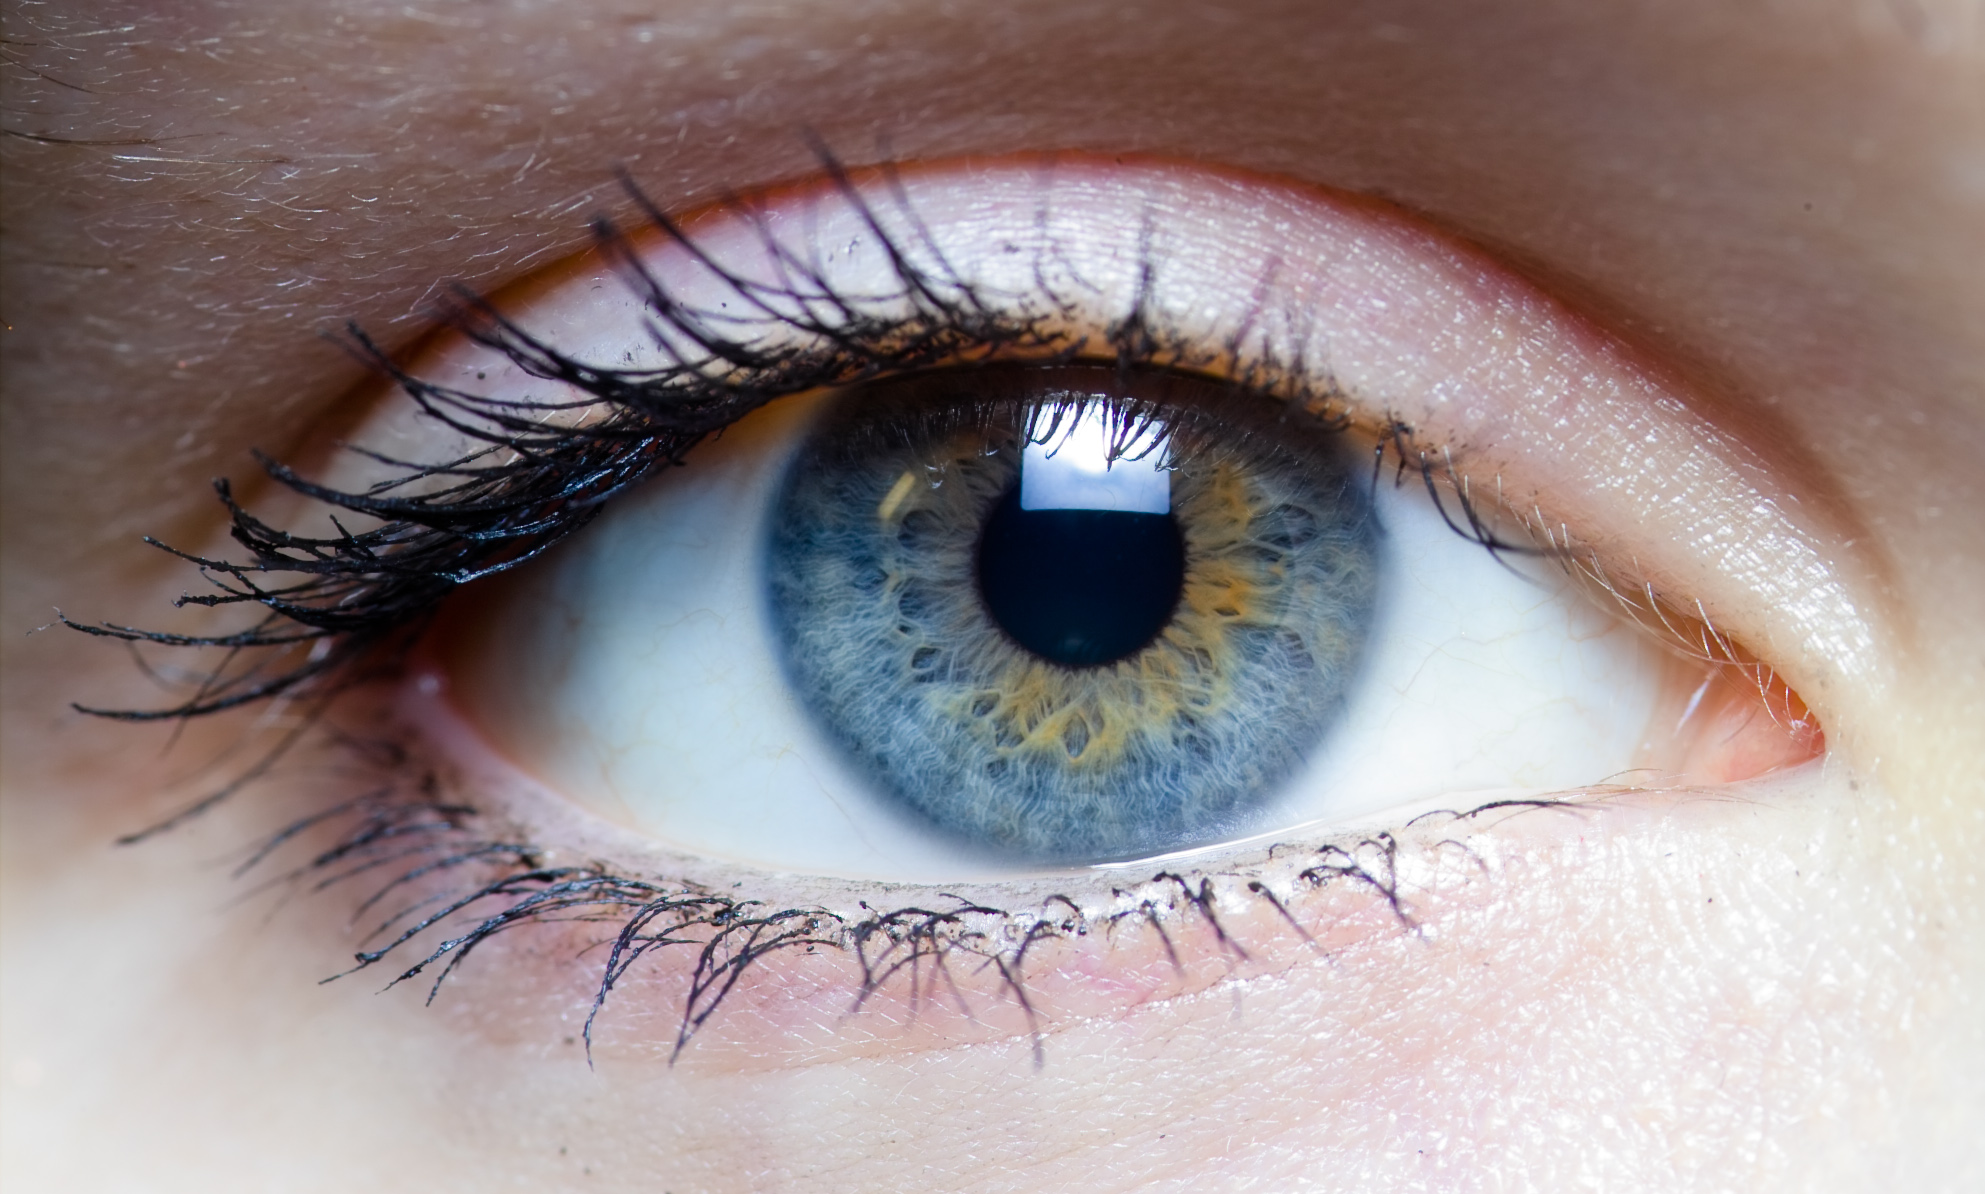
\includegraphics[width=.5\textwidth]{eye.jpg}\\
    \Large 人类的视觉感知系统存在有限的感知域
  \end{center}
\end{frame}

\begin{frame}
  \frametitle{细微变化的价值}
  \begin{center}
    \only<1>{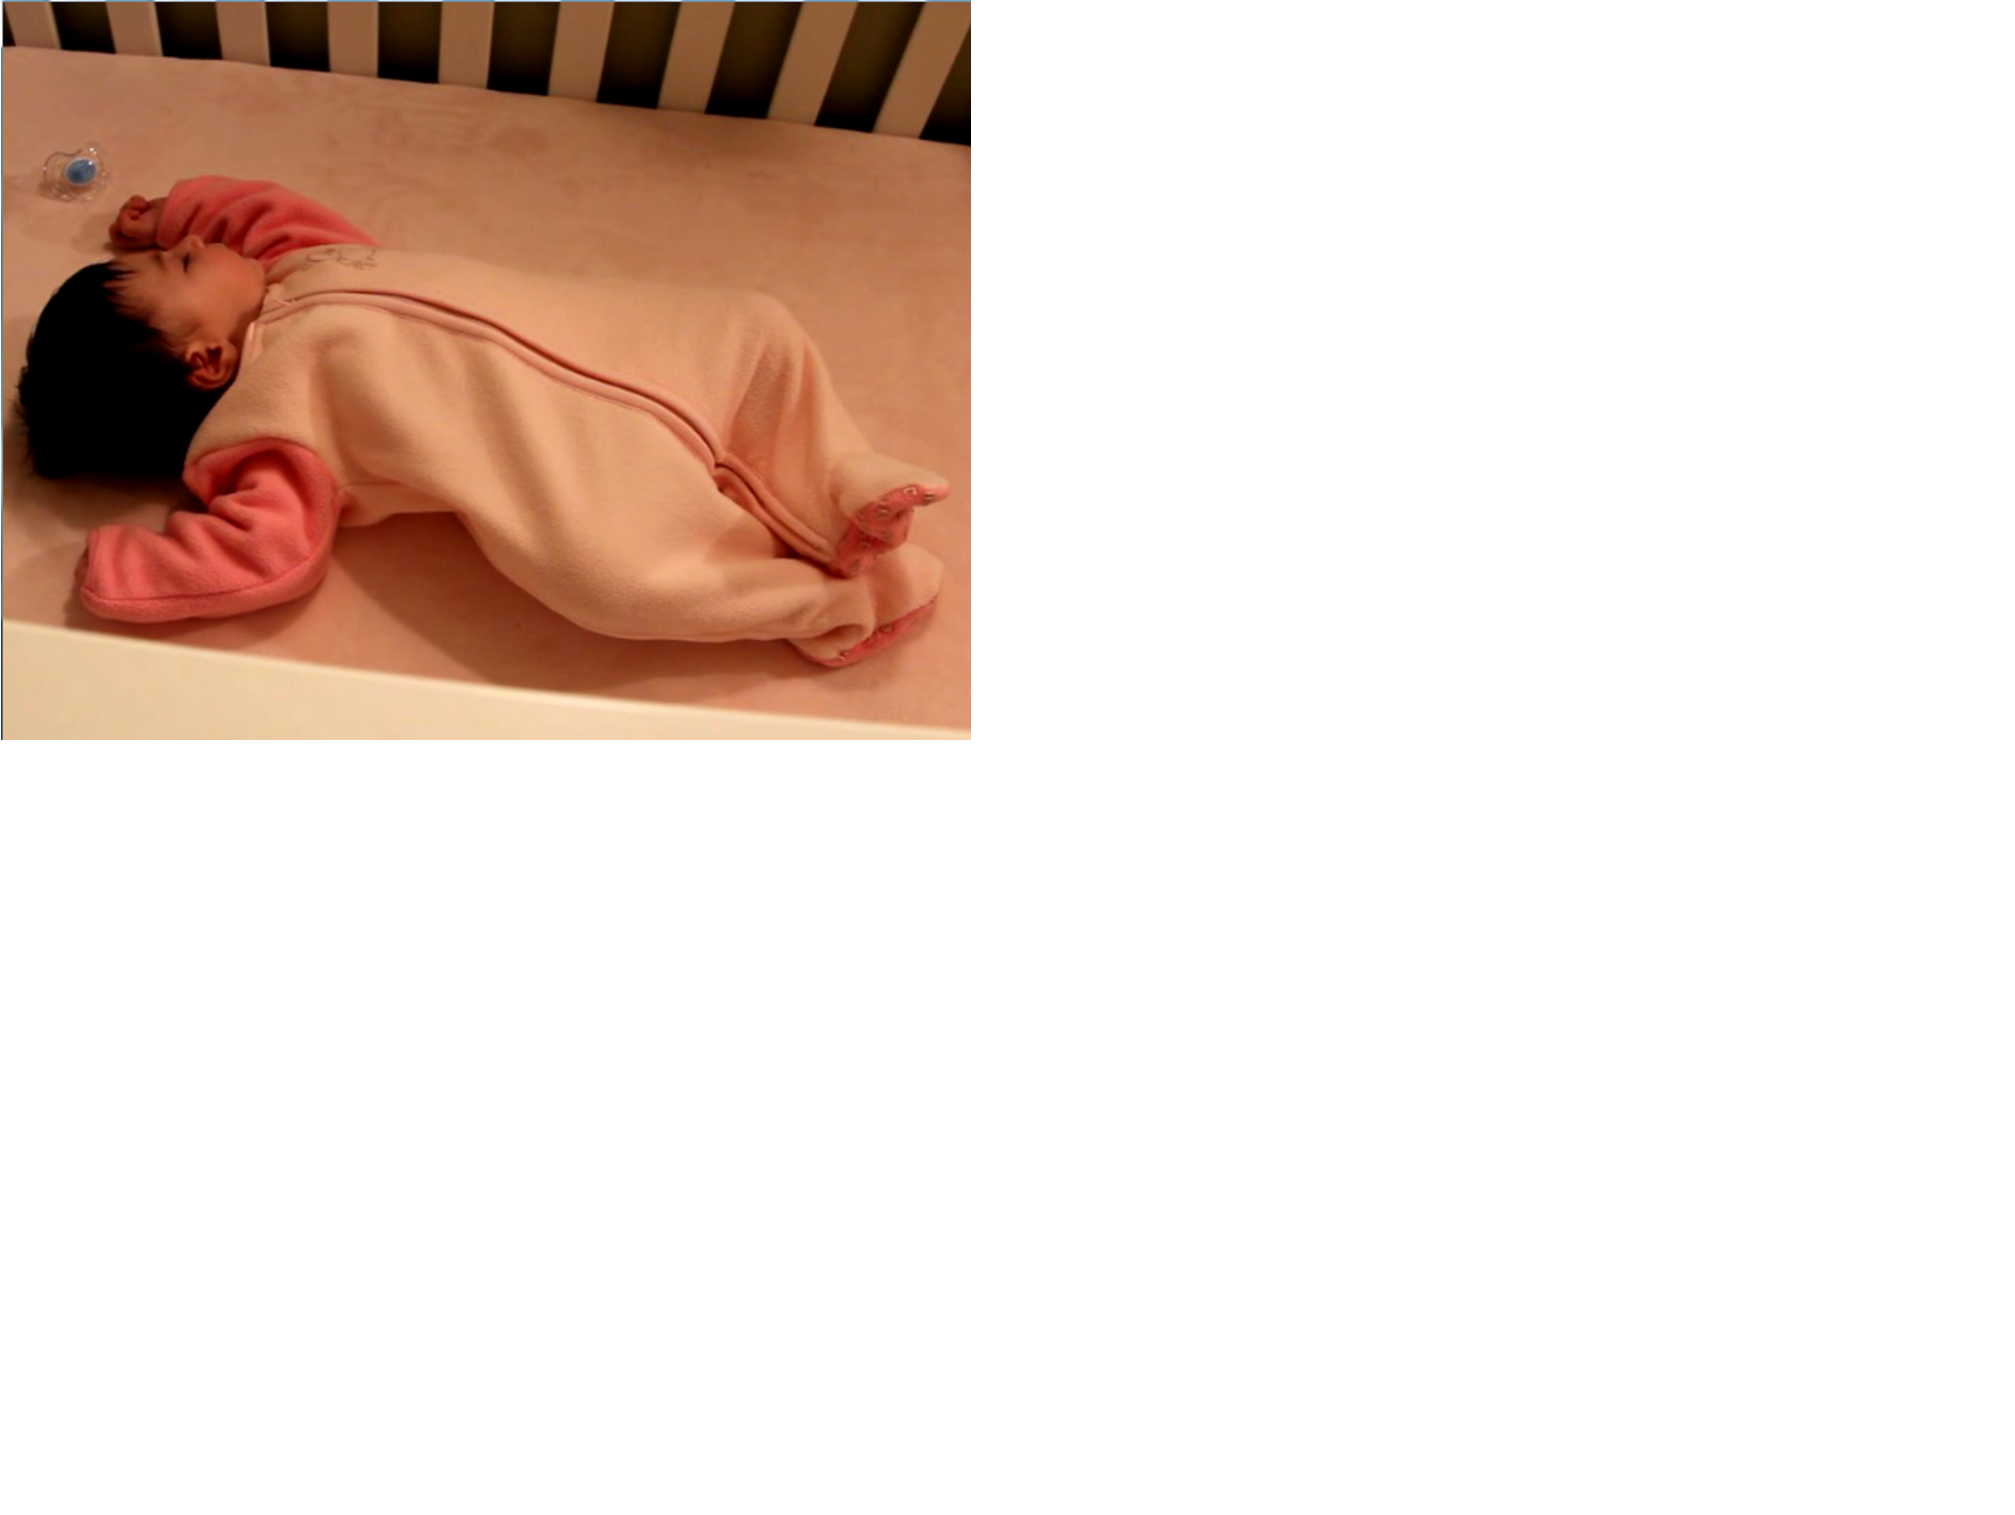
\includegraphics[width=.8\textwidth, page=1]{background/bg.pdf}}
    \only<2>{\includegraphics[width=.8\textwidth, page=2]{background/bg.pdf}}
    \only<3>{\includegraphics[width=.8\textwidth, page=3]{background/bg.pdf}}
    \only<4>{\includegraphics[width=.8\textwidth, page=4]{background/bg.pdf}}
  \end{center}
\end{frame}

\begin{frame}
  \frametitle{影像动作放大技术}
  \large
  
  影像动作放大技术是一种用于改变影像中感兴趣信号的变化幅度的技术。

  \medskip

  现有的方法\beamergotobutton{\href{./previous.mp4}{Video}}:
  \begin{itemize}
  \item 拉格朗日视角的方法:[Liu(2005)]
  \item 欧拉视角的方法:
    \begin{itemize}
    \item 线性的方法[Wu(2012)]
    \item 基于相位的方法[Wadhwa(2013)]
    \end{itemize}
  \end{itemize}
\end{frame}

\begin{frame}
  \frametitle{“鬼影”问题}

  \begin{columns}
    \Large
    \column{.5\textwidth}
    \centering
    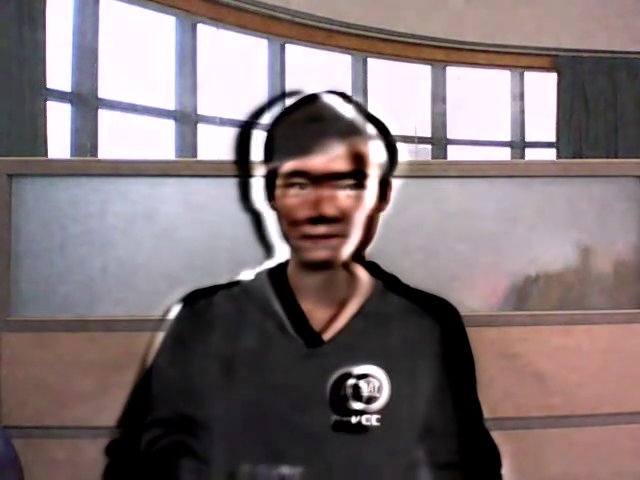
\includegraphics[width=.9\textwidth]{ghost-linear.png}\\
    线性的方法
    \column{.5\textwidth}
    \centering
    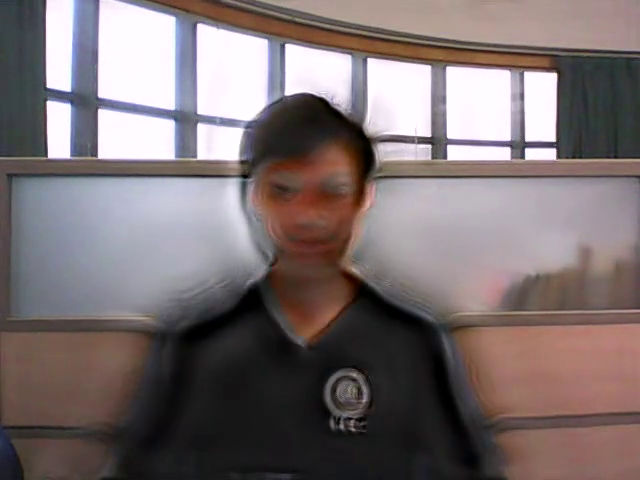
\includegraphics[width=.9\textwidth]{ghost-phase.png}\\
    基于相位的方法
  \end{columns}

  \begin{center}
    \beamergotobutton{\href{./ghost.}{Video}}
  \end{center}
\end{frame}

\section{论文主要结果}

\begin{frame}
  \frametitle{论文主要结果}
  \begin{figure}[htbp]
    \begin{tikzpicture}
      \draw[draw=white] (0,0) .. controls (3,1.3) and (6,1.3) .. (9,0)
      node[pos=0,sloped,draw=orange,inner sep=.1mm]
      {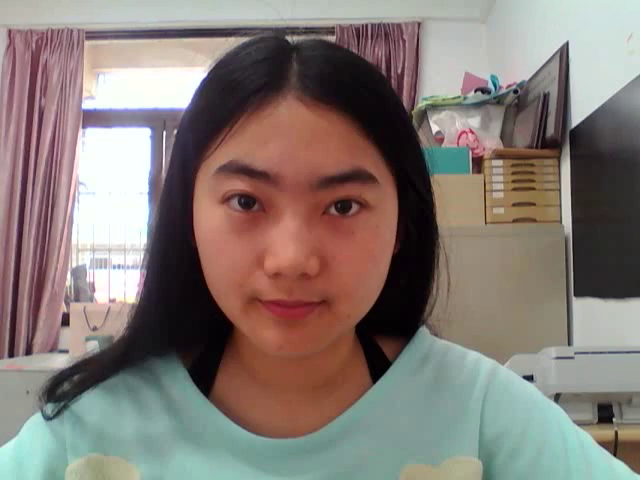
\includegraphics[height=2cm]{video1.png}}
      node[pos=0.3,sloped,draw=orange,inner sep=.1mm]
      {
\includegraphics[height=2cm]{video2.png}}
      node[pos=0.6,sloped,draw=orange,inner sep=.1mm]
      {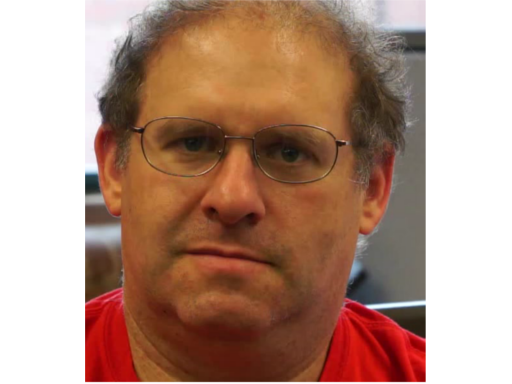
\includegraphics[height=2cm]{video3.png}}
      node[pos=0.9,sloped,draw=orange,inner sep=.1mm]
      {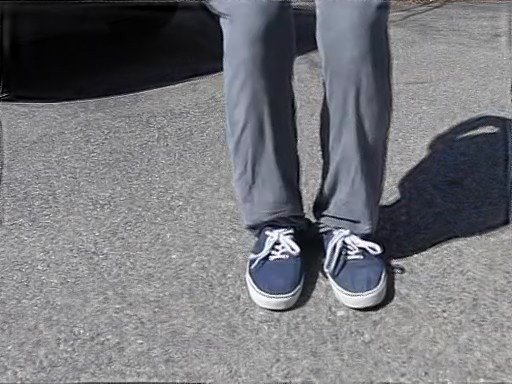
\includegraphics[height=2cm]{video4.png}};
    \end{tikzpicture}
  \end{figure}
\vspace{-2em}
\centering
\beamergotobutton{\href{./FCEVM.mp4}{video}}
\end{frame}

\begin{frame}
  \frametitle{算法框架}
  \large
  \centering
    \only<1>{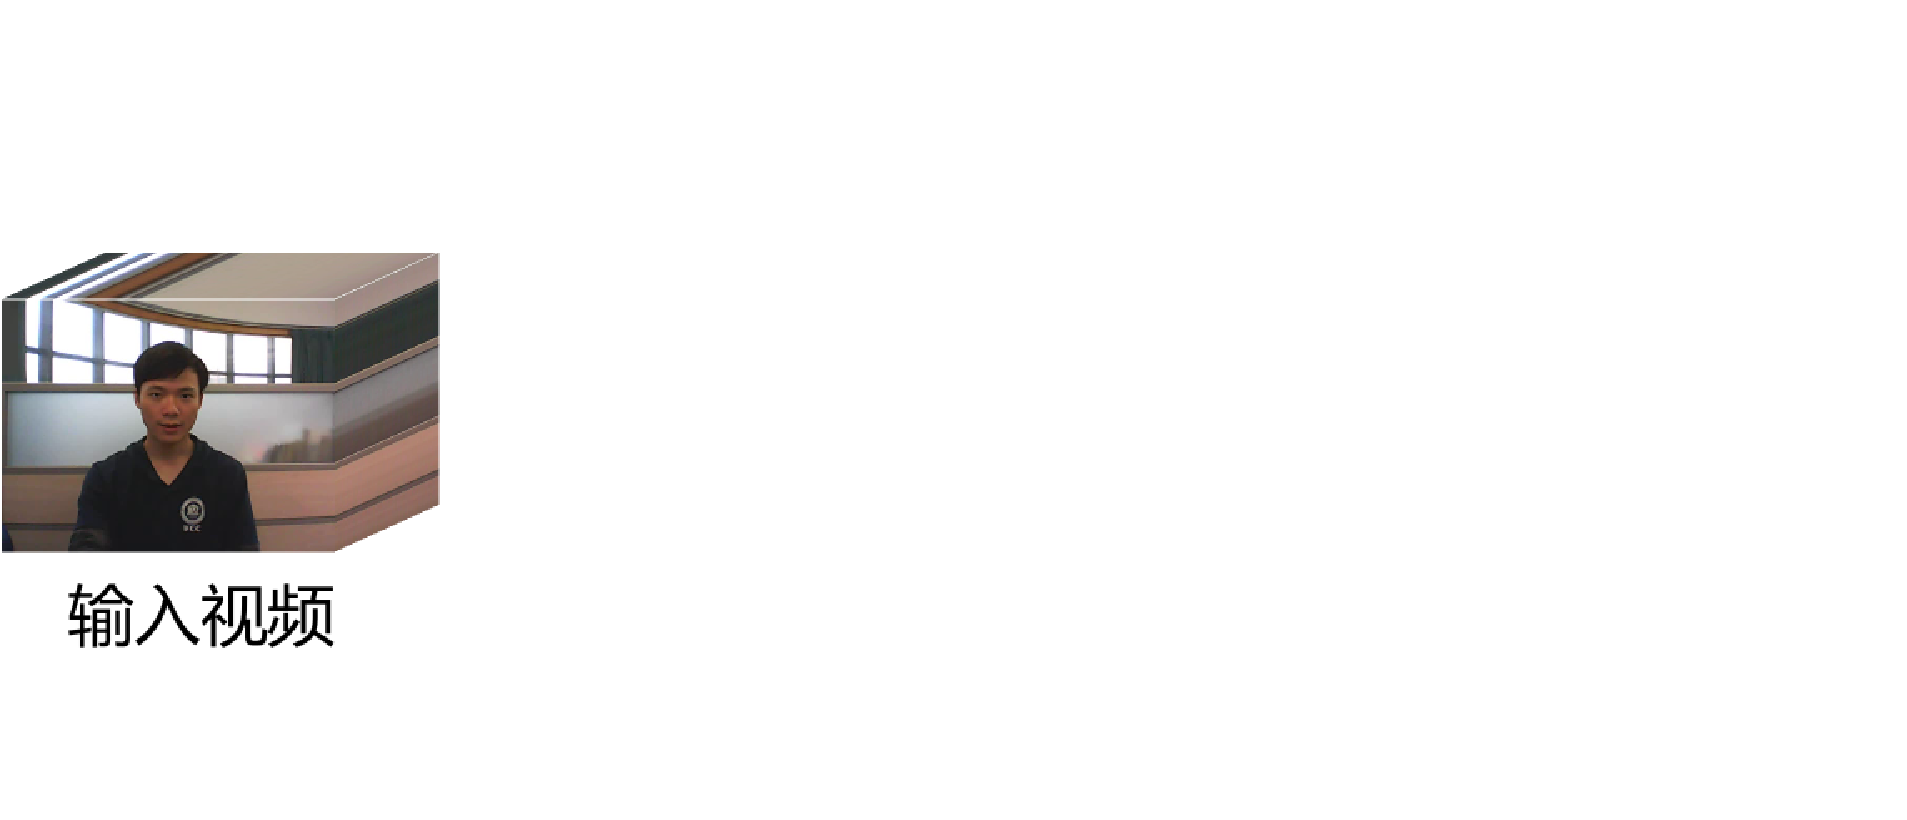
\includegraphics[width=\textwidth,
      page=1]{frameworks/frameworks.pdf}\\\medskip 输入视频}
    \only<2>{\includegraphics[width=\textwidth,
      page=2]{frameworks/frameworks.pdf}\\\medskip 用户选择感兴趣的区域}
    \only<3>{\includegraphics[width=\textwidth, page=3]{frameworks/frameworks.pdf}\\\medskip
      区域跟踪(Meanshift+Kalman),提取前景掩码(GrabCut)}
    \only<4>{\includegraphics[width=\textwidth, page=4]{frameworks/frameworks.pdf}\\\medskip 空
      间滤波}
    \only<5>{\includegraphics[width=\textwidth, page=5]{frameworks/frameworks.pdf}\\\medskip
      频域滤波(基于四元数的理想带通滤波)}
    \only<6>{\includegraphics[width=\textwidth, page=6]{frameworks/frameworks.pdf}\\\medskip 放
      大和叠加}
    \only<7>{\includegraphics[width=\textwidth, page=7]{frameworks/frameworks.pdf}\\\medskip 金
      字塔混合}
    \only<8>{\includegraphics[width=\textwidth,
      page=8]{frameworks/frameworks.pdf}\\\medskip 重构图像}
    \only<9>{\includegraphics[width=\textwidth,
      page=9]{frameworks/frameworks.pdf}\\\medskip 合成并输出视频}
\end{frame}

\section{主要创新点与待研究的问题}

\begin{frame}
  \frametitle{主要创新点}
  \Large
  \begin{itemize}[<+->]
  \item 提出了一种\alert{结合}了拉格朗日视角和欧拉视角的优点的影像动作放大方法,
    有效解决“\alert{鬼影}”问题;
  \item 基于\alert{CIEL*a*b*}颜色空间的颜色衰减;
  \item 基于\alert{四元数}的理想带通滤波。
  \end{itemize}
\end{frame}

\begin{frame}
  \frametitle{待研究的问题}
  \Large
  \begin{enumerate}[<+->]
  \item 前景分割算法的优化。
  \item 跟踪算法的增强。
  \item 引入视频校准算法。
  \end{enumerate}
\end{frame}


\begin{frame}[plain]{}
  \begin{center}
    \begin{tikzpicture}
      \node[above,xscale=1.2,yscale=1.4]{\Huge\bfseries 欢迎各位老师批评指正!};
      \node[xscale=1.2,above,yscale=-1.4,scope fading=south,opacity=0.2]{\Huge\bfseries 欢迎各位老师批评指正!};
    \end{tikzpicture}
  \end{center}
\end{frame}

\end{document}